% Chapter 3 lecture source: c3-notes.pdf :contentReference[oaicite:0]{index=0}

\section{Techniques of Integration}

\textbf{Overview.}
Chapter~1 gave us the Fundamental Theorem of Calculus: if we can find an antiderivative $F$ of $f$, then $\int_a^b f(x)\,dx=F(b)-F(a)$.
The practical difficulty is that most integrands do \emph{not} yield to a single application of the power rule or a basic substitution.
This chapter develops a toolkit of techniques---integration by parts, trigonometric identities, trigonometric substitution, partial fractions, and numerical approximation---that, taken together, let you evaluate (or at least approximate) virtually any integral that arises in MH1101.

Each technique answers a specific structural question about the integrand:

\begin{itemize}[leftmargin=*]
\item \textbf{IBP:} ``Is the integrand a \emph{product} of two functions, one of which simplifies when differentiated?''
\item \textbf{Trig integrals:} ``Does the integrand involve powers or products of trig functions that can be reduced using identities?''
\item \textbf{Trig substitution:} ``Does the integrand contain a radical $\sqrt{a^2-x^2}$, $\sqrt{a^2+x^2}$, or $\sqrt{x^2-a^2}$?''
\item \textbf{Partial fractions:} ``Is the integrand a rational function $P(x)/Q(x)$?''
\item \textbf{Numerical integration:} ``Is an antiderivative unavailable or impractical? Can we approximate the integral instead?''
\end{itemize}

\subsection{Integration by Parts}

\textbf{Motivation: reversing the Product Rule.}

We know the Product Rule for differentiation:
\[
\frac{d}{dx}\bigl(u(x)\,v(x)\bigr)=u(x)\,v'(x)+u'(x)\,v(x).
\]
This tells us how to \emph{differentiate} a product. But what if we need to \emph{integrate} a product? Rearranging the Product Rule and integrating both sides gives us a way to ``trade'' one integral for another---hopefully simpler---one.

Integrate both sides of the Product Rule over any interval (or indefinitely):
\[
u(x)\,v(x) = \int u(x)\,v'(x)\,dx + \int u'(x)\,v(x)\,dx.
\]
Solving for the first integral on the right:
\[
\int u(x)\,v'(x)\,dx = u(x)\,v(x) - \int u'(x)\,v(x)\,dx.
\]
This is the \textbf{integration-by-parts (IBP) formula}. Notice what it does: it replaces $\int u\,dv$ with $uv - \int v\,du$. The hope is that $\int v\,du$ is easier to evaluate than the original integral.

\begin{keyformula}[title={Key Formula: Integration by Parts (Indefinite and Definite)}]

The rule is the integration analogue of the Product Rule.

If $u=u(x)$ and $v=v(x)$ are differentiable, then

\[
\frac{d}{dx}\big(u(x)v(x)\big)=u(x)v'(x)+u'(x)v(x).
\]

Integrating both sides gives:

\[
\int u(x)v'(x)\,dx = u(x)v(x) - \int u'(x)v(x)\,dx.
\]

For definite integrals,

\[
\int_a^b u(x)v'(x)\,dx = \big[u(x)v(x)\big]_a^b - \int_a^b u'(x)v(x)\,dx.
\]

\end{keyformula}

\noindent
\textbf{How to choose $u$ and $dv$.}
The goal is to \emph{trade} an integral that looks hard for one that looks easier:

\[
\int \underbrace{u(x)}_{\text{differentiate}} \underbrace{dv}_{\text{integrate}}
\quad\longrightarrow\quad
u\,v - \int v\,du.
\]

A good choice typically makes:

\begin{itemize}
\item $du$ simpler than $u$ (e.g.\ polynomials shrink in degree; $\ln x$ becomes $1/x$; $\arctan x$ becomes $1/(1+x^2)$),
\item $v=\int dv$ computable immediately (avoid $dv$ whose antiderivative is unknown).
\end{itemize}

\textbf{Why the trade works (intuition).}

Think of IBP as shifting ``complexity'' from one factor to the other. If $u$ becomes simpler when differentiated (e.g.\ $x^n \to nx^{n-1}$), and $dv$ can be integrated without difficulty (e.g.\ $\sin x\,dx \to -\cos x$), then $\int v\,du$ has a \emph{simpler} first factor ($du$) multiplied by a known function ($v$). After one or more rounds of IBP, the integral may reduce to a standard form.

\begin{commonmistake}[title={Common Mistake: Forgetting the boundary term in definite IBP}]

For $\int_a^b u\,dv$, the boundary contribution $\big[uv\big]_a^b$ is \textbf{not optional}.

A frequent error is to write $\int_a^b u\,dv = uv - \int_a^b v\,du$ but forget to evaluate $uv$ at $a,b$.

\end{commonmistake}

\begin{examplebox}[title={Worked Example: $\displaystyle \int x\sin x\,dx$}]

Let $u=x$ and $dv=\sin x\,dx$. Then $du=dx$ and $v=-\cos x$. Hence

\[
\int x\sin x\,dx = uv-\int v\,du
= x(-\cos x) - \int (-\cos x)\,dx
= -x\cos x + \sin x + C.
\]

\textbf{Quick check:} Differentiate $-x\cos x+\sin x$: by the product rule we get $-\cos x+x\sin x+\cos x = x\sin x$.\ $\checkmark$

\end{examplebox}

\begin{examplebox}[title={Worked Example: $\displaystyle \int \ln x\,dx$ (why IBP is necessary)}]

There is no direct ``antiderivative rule'' for $\ln x$ itself. Treat $\ln x$ as a product:

\[
\int \ln x\,dx = \int (\ln x)\cdot 1\,dx.
\]

Choose $u=\ln x$ and $dv=dx$. Then $du=\dfrac{1}{x}\,dx$ and $v=x$. Thus

\[
\int \ln x\,dx = x\ln x - \int x\cdot \frac{1}{x}\,dx
= x\ln x - \int 1\,dx
= x\ln x - x + C.
\]

\textbf{Why this choice?} Choosing $u=\ln x$ converts $\ln x$ (which we cannot integrate directly) into $du=\frac{1}{x}\,dx$ (which combines nicely with $v=x$ to give a trivial integral $\int 1\,dx$). Choosing $u=1$ and $dv=\ln x\,dx$ would require knowing $\int \ln x\,dx$ in advance---circular!

\end{examplebox}

\begin{keyformula}[title={Key Formula: Derivatives often paired with IBP}]

These frequently appear when $u$ is an inverse trig or logarithmic function:

\[
\frac{d}{dx}(\arctan x)=\frac{1}{1+x^2},\qquad
\frac{d}{dx}(\arcsin x)=\frac{1}{\sqrt{1-x^2}},\qquad
\frac{d}{dx}(\arccos x)=-\frac{1}{\sqrt{1-x^2}}.
\]

(Use the course's standard inverse-trig derivative list when needed.)

\end{keyformula}

\textbf{Why inverse trig and log functions are always chosen as $u$:}

Functions like $\ln x$, $\arctan x$, and $\arcsin x$ are hard to integrate directly but \emph{easy to differentiate}---their derivatives are algebraic. So making them $u$ converts them into simpler $du$ terms. Meanwhile, the remaining factor (often algebraic or trigonometric) serves as $dv$ and is easy to integrate.

\begin{examplebox}[title={Worked Example: Definite IBP with a secondary substitution}]

Evaluate $\displaystyle \int_0^1 \arctan x\,dx$.

Choose $u=\arctan x$ and $dv=dx$, so $du=\dfrac{1}{1+x^2}\,dx$ and $v=x$.

Then

\begin{align*}
\int_0^1 \arctan x\,dx
&= \big[x\arctan x\big]_0^1 - \int_0^1 x\cdot \frac{1}{1+x^2}\,dx \\
&= \left(1\cdot\frac{\pi}{4}-0\right) - \int_0^1 \frac{x}{1+x^2}\,dx.
\end{align*}

For the remaining integral, set $t=1+x^2$, so $dt=2x\,dx$:

\[
\int_0^1 \frac{x}{1+x^2}\,dx = \frac12\int_{t=1}^{2}\frac{1}{t}\,dt
= \frac12\big[\ln t\big]_1^2
= \frac12\ln 2.
\]

Hence

\[
\int_0^1 \arctan x\,dx = \frac{\pi}{4}-\frac12\ln 2.
\]

\end{examplebox}

\begin{examplebox}[title={Worked Example: $\displaystyle \int x^2 e^x\,dx$ (two rounds of IBP)}]

Here the polynomial factor $x^2$ needs \emph{two} differentiations to reach $0$.

\textbf{Round 1:} Let $u=x^2$, $dv=e^x\,dx$, so $du=2x\,dx$, $v=e^x$:
\[
\int x^2 e^x\,dx = x^2 e^x - 2\int x e^x\,dx.
\]

\textbf{Round 2:} For $\int x e^x\,dx$, let $u=x$, $dv=e^x\,dx$, so $du=dx$, $v=e^x$:
\[
\int x e^x\,dx = xe^x - \int e^x\,dx = xe^x - e^x + C.
\]

Combine:
\[
\int x^2 e^x\,dx = x^2 e^x - 2(xe^x - e^x) + C = e^x(x^2-2x+2)+C.
\]

\textbf{Pattern:} Each IBP round reduces the polynomial degree by $1$. For $\int x^n e^x\,dx$, you need $n$ rounds (or use the Tabular method in the Extension below).

\end{examplebox}

\subsubsection*{Repeated integration by parts (``solve-for-the-integral'')}

\noindent
Some integrals produce the \emph{same} integral again after applying IBP. In that case, carry the repeated term to the left and solve algebraically.

\textbf{Why does the integral reappear?}

When both factors in the product ``cycle'' under differentiation and integration (e.g.\ $e^x$ stays $e^x$, while $\sin x \to \cos x \to -\sin x$), applying IBP twice brings back the original integrand. The trick is to \textbf{name} the original integral (e.g.\ $I$), and after two rounds you get an equation of the form $I = (\text{stuff}) - I$, which you solve as $2I = \text{stuff}$.

\begin{examplebox}[title={Worked Example: $\displaystyle \int e^x\sin x\,dx$ (two rounds of IBP)}]

Let

\[
I=\int e^x\sin x\,dx.
\]

First IBP: choose $u=e^x$, $dv=\sin x\,dx$. Then $du=e^x\,dx$, $v=-\cos x$:

\[
I = -e^x\cos x + \int e^x\cos x\,dx.
\]

Let $J=\int e^x\cos x\,dx$. Apply IBP again with $u=e^x$, $dv=\cos x\,dx$ so $v=\sin x$:

\[
J = e^x\sin x - \int e^x\sin x\,dx = e^x\sin x - I.
\]

Substitute into the first relation:

\[
I = -e^x\cos x + (e^x\sin x - I)
\quad\Longrightarrow\quad
2I = e^x(\sin x-\cos x).
\]

Therefore,

\[
\int e^x\sin x\,dx = \frac12 e^x(\sin x-\cos x)+C.
\]

\end{examplebox}

\begin{examtip}[title={Exam Focus: When repeated IBP is likely}]

Repeated IBP is common when the integrand is a product of:

\begin{itemize}
\item $e^{ax}$ with $\sin bx$ or $\cos bx$;
\item a polynomial with $e^{ax}$, $\sin bx$, or $\cos bx$ (eventually the polynomial differentiates to $0$).
\end{itemize}

When you see the same integral reappear, \textbf{name it} (e.g.\ $I$), then solve for $I$ explicitly.

\end{examtip}

\begin{examtip}[title={Exam Focus: Sign consistency in ``solve-for-the-integral''}]
When applying IBP twice to $\int e^{ax}\sin bx\,dx$ or $\int e^{ax}\cos bx\,dx$, you \textbf{must} use the \emph{same} choice pattern in both rounds (e.g.\ always let $u=e^{ax}$). If you switch (e.g.\ $u=e^{ax}$ in round 1 but $u=\cos bx$ in round 2), the original integral does not reappear, and you go in circles.
\end{examtip}

\newpage
\subsubsection*{Reduction formulas}

\textbf{Motivation: Why reduction formulas?}

Some families of integrals (like $\int \sin^n x\,dx$) do not have a closed-form antiderivative in terms of elementary functions for general $n$. Instead, we derive a \emph{recursive} relationship: express $\int \sin^n x\,dx$ in terms of $\int \sin^{n-2}x\,dx$. Applying this recursion repeatedly reduces the power until you reach a base case ($n=0$ or $n=1$) that you can integrate directly.

The derivation itself is just a clever IBP combined with the Pythagorean identity.

\begin{theorem}{Reduction formula for $\displaystyle \int \sin^n x\,dx$}{thm:sin-reduction}

Let $n\ge 2$ be an integer. Then

\[
\int \sin^n x\,dx
= -\frac{1}{n}\cos x\,\sin^{n-1}x+\frac{n-1}{n}\int \sin^{n-2}x\,dx.
\]

\end{theorem}

\noindent
\textbf{Proof idea (exam-usable).} Write $\sin^n x=\sin^{n-1}x\cdot \sin x$ and apply integration by parts with
$u=\sin^{n-1}x$ and $dv=\sin x\,dx$; then use $\cos^2x=1-\sin^2x$ to eliminate $\cos^2x$ and isolate the original integral on the left.

\textbf{Step-by-step derivation.}

Set $u = \sin^{n-1}x$ and $dv = \sin x\,dx$. Then $du = (n-1)\sin^{n-2}x\cos x\,dx$ and $v = -\cos x$. By IBP:
\begin{align*}
\int \sin^n x\,dx
&= -\cos x\sin^{n-1}x + (n-1)\int \sin^{n-2}x\cos^2 x\,dx.
\end{align*}
Now replace $\cos^2 x = 1 - \sin^2 x$:
\begin{align*}
\int \sin^n x\,dx
&= -\cos x\sin^{n-1}x + (n-1)\int \sin^{n-2}x\,dx - (n-1)\int \sin^n x\,dx.
\end{align*}
Move the last term to the left side:
\[
n\int \sin^n x\,dx = -\cos x\sin^{n-1}x + (n-1)\int \sin^{n-2}x\,dx.
\]
Divide by $n$ to get the stated formula.

\begin{extension}[title={Extension (Tutorial 4, Question 5, Method 1: Reduction for $\cos^n x$)}]

\textbf{Syllabus link:} Chapter 3 — \S3.1 Integration by Parts.

\textbf{Proposition.} Let $n\ge 2$ be an integer. Then

\[
\int \cos^{n}x\,dx = \frac{1}{n}\cos^{n-1}x\sin x+\frac{n-1}{n}\int \cos^{n-2}x\,dx.
\]

\textbf{Full working.}

Start from $\displaystyle \int \cos^n x\,dx=\int \cos^{n-1}x\cdot \cos x\,dx$.

Choose

\[
u=\cos^{n-1}x,\qquad dv=\cos x\,dx.
\]

Then $v=\sin x$ and

\[
du=(n-1)\cos^{n-2}x(-\sin x)\,dx=-(n-1)\cos^{n-2}x\sin x\,dx.
\]

By integration by parts,

\begin{align*}
\int \cos^n x\,dx
&= uv-\int v\,du \\
&= \cos^{n-1}x\sin x-\int \sin x\big(-(n-1)\cos^{n-2}x\sin x\big)\,dx \\
&= \cos^{n-1}x\sin x+(n-1)\int \cos^{n-2}x\sin^2 x\,dx.
\end{align*}

Use $\sin^2x=1-\cos^2x$:

\begin{align*}
\int \cos^n x\,dx
&= \cos^{n-1}x\sin x+(n-1)\int \cos^{n-2}x(1-\cos^2x)\,dx \\
&= \cos^{n-1}x\sin x+(n-1)\int \cos^{n-2}x\,dx-(n-1)\int \cos^n x\,dx.
\end{align*}

Bring the last term to the left:

\[
n\int \cos^n x\,dx=\cos^{n-1}x\sin x+(n-1)\int \cos^{n-2}x\,dx,
\]

and divide by $n$ to obtain the claimed formula.

\end{extension}

\subsubsection*{A warning on heuristics (LIATE)}

\begin{commonmistake}[title={Common Mistake: Blindly following LIATE}]

Heuristics like LIATE (Log, Inverse trig, Algebraic, Trig, Exponential) can suggest a choice for $u$, but the \textbf{actual criterion} is: does $\int v\,du$ simplify?

If a substitution is available (chain-rule structure), it often beats IBP even when LIATE ``permits'' IBP.

\end{commonmistake}

\begin{examplebox}[title={Worked Example: When substitution beats IBP}]

Evaluate $\displaystyle \int x^3\sin(x^2)\,dx$.

A fast approach is to expose a $2x\,dx$ term.

Write $x^3\,dx=x^2(x\,dx)$. Let $u=x^2$ so that $du=2x\,dx$ and $x^2=u$:

\[
\int x^3\sin(x^2)\,dx
=\frac12\int u\sin u\,du.
\]

Now apply IBP in $u$:

choose $\tilde u=u$, $d\tilde v=\sin u\,du$, so $\tilde v=-\cos u$:

\[
\frac12\int u\sin u\,du
=\frac12\Big(-u\cos u+\int \cos u\,du\Big)
=\frac12\big(-u\cos u+\sin u\big)+C.
\]

Substitute back $u=x^2$:

\[
\int x^3\sin(x^2)\,dx
=\frac12\big(-x^2\cos(x^2)+\sin(x^2)\big)+C.
\]

\end{examplebox}

\begin{extension}[title={Extension (Beyond Syllabus: Tabular Integration by Parts)}]

\textbf{Syllabus link:} Chapter 3 — \S3.1 Integration by Parts.

\textbf{Proposition (finite-derivative case).}

Let $u$ be a function such that $u^{(m+1)}(x)\equiv 0$ for some integer $m\ge 0$ (e.g.\ a polynomial of degree $m$), and let $v$ be differentiable.

Then repeated integration by parts yields

\[
\int u(x)v(x)\,dx
= \sum_{k=0}^{m}(-1)^k\,u^{(k)}(x)\,V^{(k)}(x)+C,
\]

where $V^{(0)}=\int v\,dx$ and $V^{(k)}=\int V^{(k-1)}\,dx$ (i.e.\ $V^{(k)}$ is the $k$-fold antiderivative of $v$).

\textbf{Full working (derivation).}

Apply IBP once to $\int u\,v\,dx$ with $dv=v\,dx$:

\[
\int u v\,dx = uV^{(0)}-\int u'V^{(0)}\,dx.
\]

Apply IBP again to the remaining integral:

\[
\int u'V^{(0)}\,dx = u'V^{(1)}-\int u''V^{(1)}\,dx,
\]

so

\[
\int u v\,dx = uV^{(0)}-u'V^{(1)}+\int u''V^{(1)}\,dx.
\]

Continuing this process $m$ times produces alternating signs and ends because $u^{(m+1)}\equiv 0$.

This yields the stated finite sum.

\textbf{Micro-example.}

For $\int x\cos(5x)\,dx$, take $u=x$ (so $u''=0$) and $v=\cos(5x)$.

Compute $V^{(0)}=\int \cos(5x)\,dx=\frac{1}{5}\sin(5x)$ and

$V^{(1)}=\int V^{(0)}dx=\int \frac{1}{5}\sin(5x)\,dx=-\frac{1}{25}\cos(5x)$.

Thus

\[
\int x\cos(5x)\,dx = x\cdot \frac{1}{5}\sin(5x)-1\cdot\Big(-\frac{1}{25}\cos(5x)\Big)+C
= \frac{x}{5}\sin(5x)+\frac{1}{25}\cos(5x)+C.
\]

\end{extension}

\subsection{Trigonometric Integrals}

\textbf{Motivation.}

Integrals involving powers and products of trigonometric functions arise naturally after trigonometric substitution (Section~3.3) and in Fourier analysis. The key idea: use trig identities to rewrite the integrand into a form amenable to a simple $u$-substitution or direct integration. The choice of identity depends on the \emph{parity} (odd/even) of the powers involved.

\subsubsection*{Powers of $\sin x$ and $\cos x$}

\begin{keyformula}[title={Key Formula: Power-reduction and Pythagorean identities}]

\[
\sin^2x+\cos^2x=1,\qquad
\sin^2x=\frac{1-\cos 2x}{2},\qquad
\cos^2x=\frac{1+\cos 2x}{2},\qquad
\sin x\cos x=\frac12\sin 2x.
\]

\end{keyformula}

\textbf{Why these identities?}
The Pythagorean identity $\sin^2x+\cos^2x=1$ lets you convert between $\sin$ and $\cos$ powers, which is essential when one power is odd (you ``peel off'' one factor and convert the rest). The half-angle formulas are needed when \emph{both} powers are even, because there is no odd factor to peel off; instead, you reduce the degree by expressing $\sin^2x$ or $\cos^2x$ in terms of $\cos 2x$.

\noindent
\textbf{Method-selection logic for $\int \sin^m x\cos^n x\,dx$.}

\begin{itemize}
\item If $n$ is odd: save one $\cos x$, convert the rest using $\cos^2x=1-\sin^2x$, then substitute $u=\sin x$.
\item If $m$ is odd: save one $\sin x$, convert the rest using $\sin^2x=1-\cos^2x$, then substitute $u=\cos x$.
\item If both $m,n$ are even: use power-reduction (half-angle) formulas until integrable.
\end{itemize}

\textbf{Why ``save one factor''?}

The substitution $u=\sin x$ requires $du=\cos x\,dx$, so you need exactly one leftover $\cos x$ to pair with $dx$. All remaining $\cos$ factors must be converted to $\sin$ via $\cos^2x=1-\sin^2x$, so the entire integrand becomes a polynomial in $u=\sin x$. This only works if the number of leftover $\cos$ factors after saving one is \emph{even}---which is guaranteed when $n$ is odd.

\begin{examplebox}[title={Worked Example: $\displaystyle \int \cos^3 x\,dx$ (odd power)}]

Write $\cos^3x=\cos x\cos^2x=\cos x(1-\sin^2x)$.

Let $u=\sin x$, $du=\cos x\,dx$:

\[
\int \cos^3 x\,dx
=\int (1-u^2)\,du
=u-\frac{u^3}{3}+C
=\sin x-\frac{\sin^3 x}{3}+C.
\]

\end{examplebox}

\begin{examplebox}[title={Worked Example: $\displaystyle \int \sin^5 x\cos^2 x\,dx$ (Lecture Example 3.9)}]

Since $m=5$ is odd, save one $\sin x$ and convert $\sin^4x=(\sin^2x)^2=(1-\cos^2x)^2$:
\[
\int \sin^5x\cos^2x\,dx = \int (1-\cos^2x)^2\cos^2x\sin x\,dx.
\]
Let $u=\cos x$, $du=-\sin x\,dx$:
\begin{align*}
&= -\int (1-u^2)^2 u^2\,du = -\int (u^2-2u^4+u^6)\,du\\
&= -\frac{u^3}{3}+\frac{2u^5}{5}-\frac{u^7}{7}+C
= -\frac{\cos^3x}{3}+\frac{2\cos^5x}{5}-\frac{\cos^7x}{7}+C.
\end{align*}

\end{examplebox}

\begin{examplebox}[title={Worked Example: $\displaystyle \int \sin^4 x\,dx$ (even power)}]

Use $\sin^2x=\frac{1-\cos 2x}{2}$:

\[
\sin^4x=\Big(\frac{1-\cos 2x}{2}\Big)^2
=\frac14\Big(1-2\cos 2x+\cos^2 2x\Big).
\]

Apply power-reduction again to $\cos^2 2x=\frac12(1+\cos 4x)$:

\[
\sin^4x=\frac14\Big(1-2\cos 2x+\frac12(1+\cos 4x)\Big)
=\frac14\Big(\frac32-2\cos 2x+\frac12\cos 4x\Big).
\]

Integrate term-by-term:

\[
\int \sin^4x\,dx
=\frac14\Big(\frac32 x-\sin 2x+\frac18\sin 4x\Big)+C.
\]

\end{examplebox}

\begin{examplebox}[title={Worked Example (Tutorial 5, Q1(a)): $\displaystyle \int \sin^6x\cos^3x\,dx$}]

Here $n=3$ is odd. Save one $\cos x$ and convert $\cos^2x=1-\sin^2x$:
\[
\int \sin^6x\cos^3x\,dx = \int \sin^6x(1-\sin^2x)\cos x\,dx.
\]
Let $u=\sin x$, $du=\cos x\,dx$:
\[
= \int u^6(1-u^2)\,du = \int (u^6-u^8)\,du = \frac{u^7}{7}-\frac{u^9}{9}+C
= \frac{\sin^7x}{7}-\frac{\sin^9x}{9}+C.
\]

\end{examplebox}

\subsubsection*{Powers of $\tan x$ and $\sec x$}

\begin{keyformula}[title={Key Formula: Core identity for $\tan/\sec$}]

\[
1+\tan^2x=\sec^2x,\qquad
\int \tan x\,dx=\ln|\sec x|+C,\qquad
\int \sec x\,dx=\ln|\sec x+\tan x|+C.
\]

\end{keyformula}

\textbf{Why the parallel with $\sin/\cos$?}

The identity $1+\tan^2x=\sec^2x$ plays the same role as $\sin^2x+\cos^2x=1$: it lets you convert between $\tan$ and $\sec$ powers. The key derivatives are $\frac{d}{dx}\tan x=\sec^2x$ and $\frac{d}{dx}\sec x=\sec x\tan x$, which dictate what you ``save'' for the substitution:

\begin{itemize}[leftmargin=*]
\item Save $\sec^2x\,dx$ when you want $u=\tan x$ (requires the remaining $\sec$ power to be even).
\item Save $\sec x\tan x\,dx$ when you want $u=\sec x$ (requires the remaining $\tan$ power to be even, i.e.\ original $\tan$ power is odd).
\end{itemize}

\noindent
\textbf{Method-selection logic for $\int \tan^m x\,\sec^n x\,dx$.}

\begin{itemize}
\item If $n$ is even: save a $\sec^2x$ factor, convert remaining $\sec^{n-2}x$ into $(1+\tan^2x)^{(n-2)/2}$, then substitute $u=\tan x$.
\item If $m$ is odd: save a $\sec x\tan x$ factor, convert remaining $\tan^{m-1}x$ into $(\sec^2x-1)^{(m-1)/2}$, then substitute $u=\sec x$.
\end{itemize}

\begin{examplebox}[title={Worked Example: $\displaystyle \int \tan^3x\,dx$ (reduce power)}]

Use $\tan^3x=\tan x\cdot \tan^2x=\tan x(\sec^2x-1)$:

\[
\int \tan^3x\,dx=\int \tan x\sec^2x\,dx-\int \tan x\,dx.
\]

For $\int \tan x\sec^2x\,dx$, set $u=\tan x$ so $du=\sec^2x\,dx$:

\[
\int \tan x\sec^2x\,dx=\int u\,du=\frac{u^2}{2}+C=\frac{\tan^2x}{2}+C.
\]

Hence

\[
\int \tan^3x\,dx=\frac{\tan^2x}{2}-\ln|\sec x|+C.
\]

\end{examplebox}

\begin{examplebox}[title={Worked Example (Lecture Example 3.10): $\displaystyle \int \tan^6x\sec^4x\,dx$}]

Since $n=4$ is even, save $\sec^2x$ and convert $\sec^2x=1+\tan^2x$:
\[
\int \tan^6x\sec^4x\,dx = \int \tan^6x(1+\tan^2x)\sec^2x\,dx.
\]
Let $u=\tan x$, $du=\sec^2x\,dx$:
\[
= \int u^6(1+u^2)\,du = \int(u^6+u^8)\,du = \frac{u^7}{7}+\frac{u^9}{9}+C
= \frac{\tan^7x}{7}+\frac{\tan^9x}{9}+C.
\]

\end{examplebox}

\begin{examtip}[title={Exam Focus: What if neither $m$ is odd nor $n$ is even?}]
When $m$ is even and $n$ is odd (e.g.\ $\int \sec^3x\,dx$), the standard strategies above do not directly apply. In such cases:
\begin{itemize}[leftmargin=*]
\item Try writing $\tan^mx = (\sec^2x-1)^{m/2}$ and expanding.
\item Use IBP (e.g.\ $\int \sec^3x\,dx$ is a classic IBP + solve-for-the-integral problem).
\item Use reduction formulas if available.
\end{itemize}
\end{examtip}

\subsubsection*{Product-to-sum identities}

\begin{keyformula}[title={Key Formula: Product-to-sum identities}]

\[
\sin A\cos B=\frac12\big(\sin(A-B)+\sin(A+B)\big),
\]

\[
\sin A\sin B=\frac12\big(\cos(A-B)-\cos(A+B)\big),
\]

\[
\cos A\cos B=\frac12\big(\cos(A-B)+\cos(A+B)\big).
\]

Also: $\cos(-\theta)=\cos\theta$ and $\sin(-\theta)=-\sin\theta$.

\end{keyformula}

\textbf{When to use these:}

These identities convert a \emph{product} of trig functions with \emph{different arguments} (e.g.\ $\sin 4x\cos 5x$) into a \emph{sum} of single trig functions, each of which is trivially integrable. They are \textbf{not} needed when both factors share the same argument---in that case, the power-reduction strategies above apply.

\begin{examplebox}[title={Worked Example: $\displaystyle \int \sin(4x)\cos(5x)\,dx$}]

Apply $\sin A\cos B=\frac12(\sin(A-B)+\sin(A+B))$:

\[
\sin(4x)\cos(5x)=\frac12\big(\sin(-x)+\sin(9x)\big)
=\frac12\big(-\sin x+\sin 9x\big).
\]

Thus

\[
\int \sin(4x)\cos(5x)\,dx
=\frac12\Big(\int -\sin x\,dx+\int \sin 9x\,dx\Big)
=\frac12\Big(\cos x-\frac{1}{9}\cos 9x\Big)+C.
\]

\end{examplebox}

\begin{extension}[title={Extension (Beyond Syllabus: Complex-exponential shortcut for product-to-sum)}]

\textbf{Syllabus link:} Chapter 3 — \S3.2 Trigonometric Integrals.

\textbf{Lemma (Euler).} For all real $\theta$,

\[
e^{i\theta}=\cos\theta+i\sin\theta,
\quad\text{hence}\quad
\cos\theta=\frac{e^{i\theta}+e^{-i\theta}}{2},\ \
\sin\theta=\frac{e^{i\theta}-e^{-i\theta}}{2i}.
\]

\textbf{Full working (derive $\sin A\cos B$ identity).}

Using Euler's formulas,

\[
\sin A\cos B
=\Big(\frac{e^{iA}-e^{-iA}}{2i}\Big)\Big(\frac{e^{iB}+e^{-iB}}{2}\Big)
=\frac{1}{4i}\Big(e^{i(A+B)}+e^{i(A-B)}-e^{-i(A-B)}-e^{-i(A+B)}\Big).
\]

Group the $(A\pm B)$ terms:

\[
\sin A\cos B
=\frac{1}{2}\Big(\frac{e^{i(A+B)}-e^{-i(A+B)}}{2i}+\frac{e^{i(A-B)}-e^{-i(A-B)}}{2i}\Big)
=\frac12\big(\sin(A+B)+\sin(A-B)\big).
\]

This reproduces the product-to-sum identity and provides a systematic way to derive others.

\end{extension}

\subsection{Trigonometric Substitution}

\textbf{Motivation: eliminating radicals.}

Expressions like $\sqrt{a^2-x^2}$, $\sqrt{a^2+x^2}$, and $\sqrt{x^2-a^2}$ arise frequently in geometric and physics problems (arc length, surface area, gravitational potentials). These radicals resist ordinary substitution because there is no obvious ``inner derivative'' to exploit. The idea of trigonometric substitution is to \emph{choose} a substitution that converts the radical into a pure trig expression via a Pythagorean identity, thereby eliminating the square root entirely.

For example, if we set $x=a\sin\theta$, then $a^2-x^2=a^2-a^2\sin^2\theta=a^2\cos^2\theta$, and so $\sqrt{a^2-x^2}=a\cos\theta$ (no more radical!). The integral becomes a trigonometric integral in $\theta$, which we can handle using the techniques of Section~3.2.

\begin{keyformula}[title={Key Formula: Trigonometric substitution table}]

Trigonometric substitution is designed for radicals:

\[
\sqrt{a^2-x^2},\qquad \sqrt{a^2+x^2},\qquad \sqrt{x^2-a^2}.
\]

A standard choice is:

\[
\sqrt{a^2-x^2}: \ x=a\sin\theta \ \ (-\tfrac{\pi}{2}\le\theta\le\tfrac{\pi}{2}),
\]

\[
\sqrt{a^2+x^2}: \ x=a\tan\theta \ \ (-\tfrac{\pi}{2}<\theta<\tfrac{\pi}{2}),
\]

\[
\sqrt{x^2-a^2}: \ x=a\sec\theta \ \ (0\le\theta<\tfrac{\pi}{2}\ \text{or}\ \pi\le\theta<\tfrac{3\pi}{2}).
\]

The angle restrictions make the substitution one-to-one so that $\theta$ can be expressed in terms of $x$.

\end{keyformula}

\textbf{Why these particular substitutions?}

Each substitution is chosen so that the expression under the radical becomes a perfect square of a trig function:

\begin{center}
\begin{tabular}{lll}
\textbf{Radical} & \textbf{Sub.} & \textbf{Identity used} \\
\hline
$a^2-x^2$ & $x=a\sin\theta$ & $1-\sin^2\theta=\cos^2\theta$ \\
$a^2+x^2$ & $x=a\tan\theta$ & $1+\tan^2\theta=\sec^2\theta$ \\
$x^2-a^2$ & $x=a\sec\theta$ & $\sec^2\theta-1=\tan^2\theta$ \\
\end{tabular}
\end{center}

After the substitution, $\sqrt{\cdot}$ simplifies to $a|\cos\theta|$, $a|\sec\theta|$, or $a|\tan\theta|$ respectively, and the angle restriction ensures the expression inside the absolute value is nonneg\-ative, so you can drop $|\cdot|$.

\textbf{Why the angle restrictions?}

The restriction on $\theta$ serves two purposes: (1) it makes the substitution invertible (so you can write $\theta$ back in terms of $x$ at the end), and (2) it ensures the trig function inside $\sqrt{\cdot}$ is nonneg\-ative, so you can write $\sqrt{a^2\cos^2\theta}=a\cos\theta$ (not $a|\cos\theta|$).

\noindent
\textbf{Workflow (exam-ready).}

\begin{enumerate}[label=(\arabic*)]
\item Identify the radical form and choose the matching substitution $x=g(\theta)$.
\item Compute $dx=g'(\theta)\,d\theta$ and rewrite the entire integrand in $\theta$.
\item Simplify using the identity behind the substitution (e.g.\ $1-\sin^2\theta=\cos^2\theta$).
\item Integrate in $\theta$.
\item Convert back to $x$ via a triangle (or an explicit inverse relation such as $\theta=\arcsin(x/a)$).
\end{enumerate}

\textbf{Completing the square first.}

If the expression under the radical is not already in one of the three standard forms (e.g.\ $\sqrt{5+4x-x^2}$), complete the square first: $5+4x-x^2 = 9-(x-2)^2$. Then set $u=x-2$ so the radical becomes $\sqrt{9-u^2}$, and proceed with $u=3\sin\theta$.

% Figure description (fallback): Right triangle for $x=a\sin\theta$ with hypotenuse $a$, opposite side $x$, adjacent side $\sqrt{a^2-x^2}$; used to convert $\sin\theta,\cos\theta,\tan\theta$ back to $x$.

\begin{center}
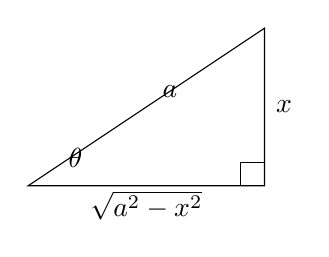
\begin{tikzpicture}[scale=1.0]
\draw (0,0) -- (3,0) -- (3,2) -- cycle;
\draw (3,0) rectangle (2.7,0.3);
\node at (1.5,-0.25) {$\sqrt{a^{2}-x^{2}}$};
\node at (3.25,1) {$x$};
\node at (1.8,1.2) {$a$};
\node at (0.6,0.35) {$\theta$};
\end{tikzpicture}
\end{center}

\begin{examplebox}[title={Worked Example: $\displaystyle \int \frac{\sqrt{9-x^2}}{x^2}\,dx$}]

Let $x=3\sin\theta$ so that $dx=3\cos\theta\,d\theta$ and

\[
\sqrt{9-x^2}=\sqrt{9-9\sin^2\theta}=3\cos\theta.
\]

Then

\[
\int \frac{\sqrt{9-x^2}}{x^2}\,dx
=\int \frac{3\cos\theta}{9\sin^2\theta}\cdot 3\cos\theta\,d\theta
=\int \frac{\cos^2\theta}{\sin^2\theta}\,d\theta
=\int \cot^2\theta\,d\theta.
\]

Use $\cot^2\theta=\csc^2\theta-1$:

\[
\int \cot^2\theta\,d\theta=\int (\csc^2\theta-1)\,d\theta
=-\cot\theta-\theta+C.
\]

Convert back. Since $x=3\sin\theta$, we have $\theta=\arcsin(x/3)$.

From the triangle, $\cot\theta=\dfrac{\sqrt{9-x^2}}{x}$.

Hence

\[
\int \frac{\sqrt{9-x^2}}{x^2}\,dx
=-\frac{\sqrt{9-x^2}}{x}-\arcsin\!\Big(\frac{x}{3}\Big)+C.
\]

\textbf{Domain check:} This answer is valid for $|x|<3$ (i.e.\ $9-x^2>0$) and $x\neq 0$.

\end{examplebox}

\begin{examplebox}[title={Worked Example (Lecture Example 3.15): Preliminary substitution + trig sub}]

Evaluate $\displaystyle \int_0^{3\sqrt3/2}\frac{x^3}{(4x^2+9)^{3/2}}\,dx$.

\textbf{Step 1:} Note $4x^2+9\neq a^2+x^2$ directly. Set $x=\frac{3}{2}\tan\theta$, so $4x^2+9=9\tan^2\theta+9=9\sec^2\theta$ and $dx=\frac{3}{2}\sec^2\theta\,d\theta$.

Limits: $x=0\Rightarrow\theta=0$; $x=\frac{3\sqrt3}{2}\Rightarrow \tan\theta=\sqrt3\Rightarrow\theta=\frac\pi3$.

\textbf{Step 2:}
\begin{align*}
\int_0^{\pi/3}\frac{(\frac32\tan\theta)^3}{(9\sec^2\theta)^{3/2}}\cdot\frac32\sec^2\theta\,d\theta
&= \int_0^{\pi/3}\frac{\frac{27}{8}\tan^3\theta}{27\sec^3\theta}\cdot\frac32\sec^2\theta\,d\theta\\
&= \frac{3}{16}\int_0^{\pi/3}\frac{\tan^3\theta}{\sec\theta}\,d\theta
= \frac{3}{16}\int_0^{\pi/3}\frac{\sin^3\theta}{\cos^2\theta}\,d\theta.
\end{align*}

\textbf{Step 3:} Write $\sin^3\theta=(1-\cos^2\theta)\sin\theta$ and let $u=\cos\theta$:
\[
\frac{3}{16}\int_1^{1/2}\frac{-(1-u^2)}{u^2}\,du
= \frac{3}{16}\int_{1/2}^{1}\Big(\frac{1}{u^2}-1\Big)\,du
= \frac{3}{16}\left[-\frac1u-u\right]_{1/2}^{1}
= \frac{3}{16}\cdot\frac{1}{2}=\frac{3}{32}.
\]

\end{examplebox}

\begin{examplebox}[title={Worked Example (Tutorial 5, Q2(c)): Completing the square + trig sub}]

Evaluate $\displaystyle \int \frac{1}{\sqrt{5+4x-x^2}}\,dx$.

\textbf{Step 1:} Complete the square: $5+4x-x^2 = 9-(x-2)^2$. Let $u=x-2$, $du=dx$:
\[
\int \frac{1}{\sqrt{9-u^2}}\,du.
\]

\textbf{Step 2:} This is a standard form: $\int\frac{du}{\sqrt{a^2-u^2}}=\arcsin\!\big(\frac{u}{a}\big)+C$ with $a=3$.
\[
= \arcsin\!\Big(\frac{u}{3}\Big)+C = \arcsin\!\Big(\frac{x-2}{3}\Big)+C.
\]

\textbf{Domain:} Valid for $|x-2|<3$, i.e.\ $-1<x<5$.

\end{examplebox}

\begin{commonmistake}[title={Common Mistake: Losing constants in the substitution}]

If the radical is $\sqrt{\alpha x^2+\beta}$, do \textbf{not} force it into $\sqrt{a^2+x^2}$ without scaling.

A standard fix is a preliminary substitution $u=\sqrt{\alpha}\,x$ so that $\alpha x^2=u^2$, then apply the trig substitution to $\sqrt{u^2+a^2}$.

\end{commonmistake}

\begin{commonmistake}[title={Common Mistake: Forgetting to convert back to $x$}]

After integrating in $\theta$, you must express the answer in terms of the original variable $x$. Draw the reference triangle:
\begin{itemize}[leftmargin=*]
\item For $x=a\sin\theta$: opposite $=x$, hypotenuse $=a$, adjacent $=\sqrt{a^2-x^2}$.
\item For $x=a\tan\theta$: opposite $=x$, adjacent $=a$, hypotenuse $=\sqrt{a^2+x^2}$.
\item For $x=a\sec\theta$: hypotenuse $=x$, adjacent $=a$, opposite $=\sqrt{x^2-a^2}$.
\end{itemize}
Read off $\sin\theta$, $\cos\theta$, $\tan\theta$, etc.\ from the triangle to complete the back-substitution.
\end{commonmistake}

\begin{examtip}[title={Exam Focus: Back-substitution sanity checks}]

After converting back to $x$:

\begin{itemize}
\item Check domain restrictions (e.g.\ $|x|\le a$ when using $x=a\sin\theta$).
\item Differentiate your final answer quickly if the integrand is algebraically delicate.
\item For definite integrals, consider switching limits to $\theta$-limits to avoid inverse trig at the end.
\end{itemize}

\end{examtip}

\subsection{Rational Functions by Partial Fractions}

\textbf{Motivation.}

A rational function $P(x)/Q(x)$ can always be integrated if we can decompose it into simpler pieces. The idea is analogous to prime factorisation for integers: just as every integer factors uniquely into primes, every polynomial over $\mathbb{R}$ factors into linear and irreducible quadratic factors. We then ``un-add'' the fraction into a sum of simpler fractions (partial fractions), each of which has a known antiderivative.

\textbf{Why must the fraction be proper first?}

A proper fraction ($\deg P < \deg Q$) decomposes into partial fractions that are genuinely ``simpler'' (each has degree of numerator strictly less than degree of denominator factor). If the fraction is \emph{improper}, polynomial long division extracts the polynomial part first; the remainder is then proper and can be decomposed.

\begin{definition}{Rational function and properness}{def:rational}

A \textbf{rational function} is a ratio of polynomials:

\[
\frac{P(x)}{Q(x)}\qquad (Q(x)\neq 0).
\]

It is \textbf{proper} if $\deg P<\deg Q$. If not proper, perform polynomial long division first to rewrite it as

\[
\frac{P(x)}{Q(x)} = S(x) + \frac{R(x)}{Q(x)},
\quad \deg R<\deg Q.
\]

\end{definition}

\begin{keyformula}[title={Key Formula: Partial fraction templates}]

Factor $Q(x)$ over $\mathbb{R}$ into linear and irreducible quadratic factors.

\begin{itemize}
\item Linear factor $(ax+b)^r$ contributes

\[
\frac{A_1}{ax+b}+\frac{A_2}{(ax+b)^2}+\cdots+\frac{A_r}{(ax+b)^r}.
\]

\item Irreducible quadratic factor $(ax^2+bx+c)^r$ contributes

\[
\frac{A_1x+B_1}{ax^2+bx+c}+\frac{A_2x+B_2}{(ax^2+bx+c)^2}+\cdots+\frac{A_rx+B_r}{(ax^2+bx+c)^r}.
\]

\end{itemize}

\end{keyformula}

\textbf{Why the different numerator forms?}

Each partial fraction must be proper with respect to its own denominator factor:
\begin{itemize}[leftmargin=*]
\item Over a \emph{linear} factor $(ax+b)^k$ (degree 1), a proper numerator has degree $<1$, so it is a constant $A$.
\item Over an \emph{irreducible quadratic} $(ax^2+bx+c)^k$ (degree 2), a proper numerator has degree $<2$, so it is linear: $Ax+B$.
\end{itemize}
Using a constant over an irreducible quadratic would leave you with too few unknowns to match all coefficients of $P(x)$---the system would be inconsistent.

\noindent
\textbf{Integration after decomposition.}

\begin{itemize}
\item Terms $\dfrac{1}{ax+b}$ integrate to $\ln|ax+b|$.
\item Terms $\dfrac{1}{(ax+b)^k}$ integrate by power rule.
\item For $\dfrac{Ax+B}{ax^2+bx+c}$, split into a derivative-of-denominator part plus a remainder:

\[
Ax+B = \lambda(2ax+b) + \mu,
\]

so that $\int \dfrac{\lambda(2ax+b)}{ax^2+bx+c}\,dx$ is logarithmic, while

$\int \dfrac{\mu}{ax^2+bx+c}\,dx$ uses completing the square and $\arctan$.

\end{itemize}

\textbf{Why the ``derivative of denominator'' trick?}

If the numerator is a constant multiple of $Q'(x)=2ax+b$, then the integral is simply $\lambda\ln|Q(x)|+C$ (by substitution $u=Q(x)$). So we deliberately decompose $Ax+B$ into a multiple of $Q'(x)$ plus a leftover constant. The leftover gives an $\arctan$ after completing the square.

\begin{examplebox}[title={Worked Example: Proper rational function (linear factors)}]

Evaluate $\displaystyle \int \frac{x^{2}+2x-1}{2x^{3}+3x^{2}-2x}\,dx$.

First factor the denominator:

\[
2x^{3}+3x^{2}-2x=x(2x^{2}+3x-2)=x(2x-1)(x+2).
\]

So write

\[
\frac{x^{2}+2x-1}{x(2x-1)(x+2)}=\frac{A}{x}+\frac{B}{2x-1}+\frac{C}{x+2}.
\]

Multiply through by $x(2x-1)(x+2)$:

\[
x^{2}+2x-1 = A(2x-1)(x+2)+Bx(x+2)+Cx(2x-1).
\]

Expanding and matching coefficients yields $A=\frac12$, $B=\frac15$, $C=-\frac{1}{10}$, hence

\[
\int \frac{x^{2}+2x-1}{2x^{3}+3x^{2}-2x}\,dx
=\int\Big(\frac{1}{2x}+\frac{1}{5(2x-1)}-\frac{1}{10(x+2)}\Big)\,dx.
\]

Integrate term-by-term:

\[
=\frac12\ln|x|+\frac{1}{10}\ln|2x-1|-\frac{1}{10}\ln|x+2|+C.
\]

\end{examplebox}

\begin{examplebox}[title={Worked Example: Improper rational function (long division first)}]

Evaluate $\displaystyle \int \frac{x^{4}-2x^{2}+4x+1}{x^{3}-x^{2}-x+1}\,dx$.

Since $\deg$ numerator $>\deg$ denominator, do long division:

\[
\frac{x^{4}-2x^{2}+4x+1}{x^{3}-x^{2}-x+1}
= x+1+\frac{4x}{x^{3}-x^{2}-x+1}.
\]

Factor $x^{3}-x^{2}-x+1$. Since $Q(1)=0$, $(x-1)$ is a factor, and

\[
x^{3}-x^{2}-x+1=(x-1)^{2}(x+1).
\]

Decompose

\[
\frac{4x}{(x-1)^{2}(x+1)}=\frac{A}{x-1}+\frac{B}{(x-1)^{2}}+\frac{C}{x+1}.
\]

Solving gives $A=1$, $B=2$, $C=-1$, so

\[
\frac{x^{4}-2x^{2}+4x+1}{x^{3}-x^{2}-x+1}
= x+1+\frac{1}{x-1}+\frac{2}{(x-1)^{2}}-\frac{1}{x+1}.
\]

Integrate:

\[
\int \Big(x+1\Big)\,dx=\frac{x^{2}}{2}+x,\quad
\int \frac{1}{x-1}\,dx=\ln|x-1|,
\]

\[
\int \frac{2}{(x-1)^{2}}\,dx = 2\int (x-1)^{-2}\,dx = -\frac{2}{x-1},\quad
\int \frac{1}{x+1}\,dx=\ln|x+1|.
\]

Thus

\[
\int \frac{x^{4}-2x^{2}+4x+1}{x^{3}-x^{2}-x+1}\,dx
=\frac{x^{2}}{2}+x-\frac{2}{x-1}+\ln\Big|\frac{x-1}{x+1}\Big|+C.
\]

\end{examplebox}

\begin{examplebox}[title={Worked Example (Tutorial 6, Q1(b)): Irreducible quadratic in the denominator}]

Evaluate $\displaystyle \int \frac{4x}{x^3+x^2+x+1}\,dx$.

\textbf{Step 1: Factor.} $x^3+x^2+x+1 = x^2(x+1)+(x+1) = (x+1)(x^2+1)$.

Note $x^2+1$ is irreducible over $\mathbb{R}$ (discriminant $<0$).

\textbf{Step 2: Decompose.}
\[
\frac{4x}{(x+1)(x^2+1)} = \frac{A}{x+1}+\frac{Bx+C}{x^2+1}.
\]
Multiply through: $4x = A(x^2+1)+(Bx+C)(x+1)$.

Set $x=-1$: $-4=2A$, so $A=-2$.

Expand and compare $x^2$-coefficients: $0=A+B=-2+B$, so $B=2$.

Compare constant terms: $0=A+C=-2+C$, so $C=2$.

\textbf{Step 3: Integrate.}
\begin{align*}
\int \frac{4x}{(x+1)(x^2+1)}\,dx
&= \int\left(\frac{-2}{x+1}+\frac{2x+2}{x^2+1}\right)\,dx\\
&= -2\ln|x+1| + \int\frac{2x}{x^2+1}\,dx + 2\int\frac{1}{x^2+1}\,dx\\
&= -2\ln|x+1| + \ln(x^2+1) + 2\arctan x + C.
\end{align*}

\textbf{Note:} The $\frac{2x}{x^2+1}$ term integrates as $\ln(x^2+1)$ because $2x$ is the derivative of $x^2+1$---exactly the ``derivative of denominator'' trick.

\end{examplebox}

\begin{examplebox}[title={Worked Example (Tutorial 6, Q1(e)): Exponential rational integral}]

Evaluate $\displaystyle \int \frac{e^{2x}}{e^{2x}+3e^x+2}\,dx$.

\textbf{Key idea:} Let $u=e^x$ ($u>0$), $du=e^x\,dx$. Then $e^{2x}=u^2$ and $dx=\frac{du}{u}$:
\[
\int \frac{u^2}{u^2+3u+2}\cdot\frac{du}{u} = \int \frac{u}{(u+1)(u+2)}\,du.
\]

Decompose: $\frac{u}{(u+1)(u+2)}=\frac{-1}{u+1}+\frac{2}{u+2}$.

Integrate:
\[
= -\ln|u+1|+2\ln|u+2|+C = -\ln(e^x+1)+2\ln(e^x+2)+C.
\]

(Since $u=e^x>0$, absolute values are unnecessary.)

\end{examplebox}

\begin{commonmistake}[title={Common Mistake: Missing $(Ax+B)$ over an irreducible quadratic}]

If $x^2+1$ (or any irreducible quadratic) appears in the denominator, the numerator of its partial fraction term must be linear ($Ax+B$), not a constant.

Otherwise you will not have enough degrees of freedom to match coefficients.

\end{commonmistake}

\begin{commonmistake}[title={Common Mistake: Forgetting long division for improper fractions}]
If $\deg P \ge \deg Q$, you \textbf{must} do long division before decomposing. Setting up partial fractions on an improper fraction gives an inconsistent system of equations.

\textbf{Quick degree check:} look at the leading terms of $P$ and $Q$. If the degree of $P$ is at least the degree of $Q$, divide first.
\end{commonmistake}

\begin{examtip}[title={Exam Focus: Efficient coefficient-finding strategies}]
\begin{itemize}[leftmargin=*]
\item \textbf{Strategic substitution:} After multiplying both sides by $Q(x)$, plug in the roots of $Q$ to isolate one unknown at a time (this is the Heaviside cover-up idea for distinct linear factors).
\item \textbf{Coefficient matching:} For repeated or quadratic factors where strategic substitution alone does not determine all unknowns, expand and compare coefficients of $x^k$.
\item \textbf{Hybrid:} Use strategic substitution for as many unknowns as possible, then compare one or two coefficients for the rest.
\end{itemize}
\end{examtip}

\begin{extension}[title={Extension (Beyond Syllabus: Heaviside cover-up for distinct linear factors)}]

\textbf{Syllabus link:} Chapter 3 — \S3.4 Rational Functions by Partial Fractions.

\textbf{Proposition (cover-up method).}

Suppose a rational function has the form

\[
\frac{P(x)}{\prod_{k=1}^{m}(x-a_k)}
=\sum_{k=1}^{m}\frac{A_k}{x-a_k},
\]

where the $a_k$ are \emph{distinct} (no repeated roots) and $\deg P<m$. Then each coefficient is

\[
A_j = \left.\frac{P(x)}{\prod_{k\neq j}(x-a_k)}\right|_{x=a_j}.
\]

\textbf{Full working (why it works).}

Multiply both sides by $\prod_{k=1}^{m}(x-a_k)$:

\[
P(x)=\sum_{k=1}^{m}A_k\,\prod_{\ell\neq k}(x-a_\ell).
\]

Now set $x=a_j$. Every term with $k\neq j$ contains a factor $(a_j-a_j)=0$ and vanishes, leaving

\[
P(a_j) = A_j\,\prod_{\ell\neq j}(a_j-a_\ell),
\]

so $A_j = \dfrac{P(a_j)}{\prod_{\ell\neq j}(a_j-a_\ell)}
= \left.\dfrac{P(x)}{\prod_{k\neq j}(x-a_k)}\right|_{x=a_j}$.

\textbf{Micro-example.}

For $\dfrac{x+5}{(x-1)(x+2)}=\dfrac{A}{x-1}+\dfrac{B}{x+2}$:

Cover up $(x-1)$ and set $x=1$: $A = \dfrac{1+5}{1+2}=2$.

Cover up $(x+2)$ and set $x=-2$: $B = \dfrac{-2+5}{-2-1}=-1$.

\end{extension}

\subsection{Numerical Integration I: Midpoint and Trapezoidal Rules}

\textbf{Motivation: when antiderivatives fail.}

Not every function has a ``nice'' closed-form antiderivative. For instance, $\int e^{-x^2}\,dx$ cannot be expressed in terms of elementary functions. Even when an antiderivative exists, it may be so complicated that numerical approximation is more practical. The idea is to go back to the \emph{definition} of the definite integral as a limit of Riemann sums and use finite sums as approximations.

\textbf{Riemann-sum viewpoint.}

When an antiderivative is hard or unavailable, we approximate $\int_a^b f(x)\,dx$ using Riemann sums. Partition $[a,b]$ into $n$ equal subintervals with $\Delta x=\frac{b-a}{n}$, $x_i=a+i\,\Delta x$ ($i=0,1,\ldots,n$).

A general Riemann-sum approximation is

\[
\int_a^b f(x)\,dx \approx \sum_{i=1}^n f(x_i^*)\,\Delta x,
\]

where $x_i^*\in[x_{i-1},x_i]$. Different choices of $x_i^*$ yield different rules.

\textbf{Why different rules?}

\begin{itemize}[leftmargin=*]
\item \textbf{Left/Right endpoints} ($L_n$/$R_n$): simplest but least accurate. They are first-order methods (error $\sim 1/n$).
\item \textbf{Midpoint rule} ($M_n$): uses the midpoint of each subinterval. Surprisingly, this is more accurate than endpoints because errors on the left and right halves of each subinterval partially cancel. It is second-order (error $\sim 1/n^2$).
\item \textbf{Trapezoidal rule} ($T_n$): averages $L_n$ and $R_n$, which is equivalent to approximating $f$ by a straight line (trapezoid) on each subinterval. Also second-order, but typically about twice the error of the midpoint rule.
\end{itemize}

\begin{keyformula}[title={Key Formula: Endpoint, Midpoint, and Trapezoidal rules}]

\textbf{Left endpoints:}\quad $L_n = \displaystyle\sum_{i=1}^{n}f(x_{i-1})\,\Delta x$.

\textbf{Right endpoints:}\quad $R_n = \displaystyle\sum_{i=1}^{n}f(x_i)\,\Delta x$.

\textbf{Midpoint rule:}\quad $M_n = \displaystyle\sum_{i=1}^{n}f\!\Big(\frac{x_{i-1}+x_i}{2}\Big)\,\Delta x$.

\textbf{Trapezoidal rule:}\quad $T_n = \dfrac{L_n+R_n}{2} = \dfrac{\Delta x}{2}\Big(f(x_0)+2f(x_1)+2f(x_2)+\cdots+2f(x_{n-1})+f(x_n)\Big)$.

\end{keyformula}

\textbf{Why is $T_n$ the average of $L_n$ and $R_n$?}

On each subinterval $[x_{i-1},x_i]$, $L_n$ uses the left height $f(x_{i-1})$ and $R_n$ uses the right height $f(x_i)$. Their average gives $\frac{f(x_{i-1})+f(x_i)}{2}\cdot\Delta x$, which is exactly the area of a \emph{trapezoid} with parallel sides $f(x_{i-1})$ and $f(x_i)$ and width $\Delta x$. Summing over all subintervals gives the formula above, with the interior $f(x_i)$ values counted twice (they are shared by adjacent trapezoids) and the endpoints counted once.

\begin{examplebox}[title={Worked Example: $T_5$ and $M_5$ for $\displaystyle\int_1^2\frac{1}{x}\,dx$}]

Let $f(x)=\frac1x$, $a=1$, $b=2$, $n=5$, so $\Delta x=0.2$ and $x_0=1$, $x_1=1.2$, $x_2=1.4$, $x_3=1.6$, $x_4=1.8$, $x_5=2$.

\textbf{Trapezoidal rule:}

$T_5=\frac{0.2}{2}\big(f(x_0)+2f(x_1)+2f(x_2)+2f(x_3)+2f(x_4)+f(x_5)\big)$.

Substitute values:

$T_5 = 0.1\left(1+\frac{2}{1.2}+\frac{2}{1.4}+\frac{2}{1.6}+\frac{2}{1.8}+\frac12\right)\approx 0.695635$.

\textbf{Midpoint rule} uses midpoints $1.1,1.3,1.5,1.7,1.9$:

$M_5=0.2\left(\frac{1}{1.1}+\frac{1}{1.3}+\frac{1}{1.5}+\frac{1}{1.7}+\frac{1}{1.9}\right)\approx 0.691908$.

For reference, the exact value is $\int_1^2\frac1x\,dx = \ln 2 \approx 0.693147$.

\textbf{Observation:} $M_5$ is closer to the exact value than $T_5$. This is typical: the midpoint rule error is roughly half the trapezoidal rule error.

\end{examplebox}

\subsubsection*{Error bounds}

\textbf{Why error bounds matter.}

Computing $T_n$ or $M_n$ gives a number, but how close is it to the true integral? The error bounds below answer: ``how large must $n$ be to guarantee accuracy to $k$ decimal places?'' They depend on $|f''(x)|$, which measures how ``curved'' $f$ is---the more curved, the worse a piecewise-linear (trapezoidal) or piecewise-constant (midpoint) approximation performs.

\begin{definition}{Approximation errors}{def:numerical-errors}

Define the errors

$E_T=\int_a^b f(x)\,dx - T_n$,\quad
$E_M=\int_a^b f(x)\,dx - M_n$,

and similarly $E_L=\int_a^b f(x)\,dx-L_n$, $E_R=\int_a^b f(x)\,dx-R_n$.

\end{definition}

\begin{theorem}{Error bounds for Trapezoidal and Midpoint rules}{thm:trap-mid-error}

Assume $f''$ is twice differentiable on $[a,b]$ and $|f''(x)|\le K$ for all $x\in[a,b]$. Then

\[
|E_T| \le \frac{K(b-a)^3}{12n^2},\qquad
|E_M| \le \frac{K(b-a)^3}{24n^2}.
\]

\end{theorem}

\textbf{Observations from the bounds:}
\begin{itemize}[leftmargin=*]
\item The midpoint bound has $24$ in the denominator vs.\ $12$ for the trapezoidal rule, so the midpoint error bound is \emph{half} as large. This matches the empirical observation.
\item Both errors decrease as $1/n^2$: doubling $n$ reduces the error by a factor of $4$.
\item The bound involves $K = \max|f''|$: for nearly-linear functions ($f''\approx 0$), both rules are very accurate.
\end{itemize}

\begin{examtip}[title={Exam Focus: Using error bounds efficiently}]

To guarantee an accuracy target:

\begin{itemize}
\item Compute or bound $|f''(x)|$ on $[a,b]$ and choose a valid $K$ (often the maximum occurs at an endpoint).
\item Solve the inequality from the relevant bound for $n$.
\item Round up to the next integer since $n$ must be an integer.
\end{itemize}

\end{examtip}

\begin{examplebox}[title={Worked Example: Choose $n$ for midpoint accuracy}]

Find $n$ such that $M_n$ approximates $\int_1^4\sqrt{x}\,dx$ with error at most $10^{-4}$.

Let $f(x)=\sqrt{x}=x^{1/2}$. Then $f'(x)=\frac12 x^{-1/2}$, $f''(x)=-\frac14 x^{-3/2}$, $|f''(x)|=\frac14 x^{-3/2}$.

On $[1,4]$, $x^{-3/2}$ decreases, so the maximum occurs at $x=1$: $|f''(x)|\le \frac14 = K$.

Apply the midpoint bound:

\[
|E_M| \le \frac{K(b-a)^3}{24n^2} = \frac{\frac14\cdot 3^3}{24n^2} = \frac{27}{96n^2} \le 10^{-4}.
\]

So $n^2 \ge \frac{27}{96}\cdot 10^4 = 2812.5$, hence $n \ge \sqrt{2812.5}\approx 53.033$.

Thus $n=54$ suffices.

\end{examplebox}

\begin{examplebox}[title={Worked Example (Tutorial 6, Q2): $T_8$, $M_8$ and error for $\int_0^1 e^{-x^2}\,dx$}]

Let $f(x)=e^{-x^2}$, $a=0$, $b=1$, $n=8$, $\Delta x = 1/8$.

\textbf{(a) Compute $T_8$ and $M_8$.}

$T_8 = \frac{1/8}{2}\bigl(f(0)+2f(1/8)+\cdots+2f(7/8)+f(1)\bigr)$.

$M_8 = \frac18\bigl(f(1/16)+f(3/16)+\cdots+f(15/16)\bigr)$.

(Numerical evaluation gives $T_8\approx 0.902333$, $M_8\approx 0.905620$ using $f(x)=e^{-x^2}$; the exact value is $\approx 0.746824$---but for the tutorial function $f(x)=e^{x^2}$ on $[0,1]$, the exact value is different. Substitute the actual function values as specified.)

\textbf{(b) Error estimation.}

$f'(x) = -2xe^{-x^2}$, $f''(x) = (4x^2-2)e^{-x^2}$.

On $[0,1]$: $|f''(x)| = |4x^2-2|\,e^{-x^2} \le 2e^0 = 2$ at $x=0$. (Check boundary and critical points.) Take $K=6$ as a safe bound (tutorial uses $K=6$).

Then $|E_T|\le \frac{6}{12\cdot 64}\approx 0.0078$ and $|E_M|\le \frac{6}{24\cdot 64}\approx 0.0039$.

\textbf{(c) For accuracy $10^{-4}$:} $\frac{K}{12n^2}\le 10^{-4}$ gives $n\ge 71$ (trapezoidal); $\frac{K}{24n^2}\le 10^{-4}$ gives $n\ge 50$ (midpoint).

\end{examplebox}

\begin{commonmistake}[title={Common Mistake: Choosing $K$ incorrectly}]
$K$ is a bound on $|f''(x)|$ over $[a,b]$. You need the \textbf{maximum} of $|f''|$, not just $|f''(a)|$ or $|f''(b)|$.
\begin{itemize}[leftmargin=*]
\item If $|f''|$ is monotone on $[a,b]$, the max occurs at an endpoint.
\item If $|f''|$ has interior critical points, find them (solve $f'''(x)=0$) and compare values.
\item It is fine to \emph{overestimate} $K$---this gives a slightly larger $n$ than necessary, which is conservative but safe.
\end{itemize}
\end{commonmistake}

\subsection{Numerical Integration II: Simpson's Rule}

\textbf{Motivation: can we do better than $O(1/n^2)$?}

The trapezoidal and midpoint rules approximate $f$ by straight lines (degree-1 polynomials) on each subinterval, giving error $\sim 1/n^2$. Simpson's Rule approximates $f$ by \emph{parabolas} (degree-2 polynomials) on pairs of subintervals, and achieves error $\sim 1/n^4$---a dramatic improvement. Doubling $n$ now reduces the error by a factor of $16$ instead of $4$.

\textbf{Definition and derivation as a weighted average.}

Simpson's Rule combines the trapezoidal and midpoint ideas on pairs of subintervals. From our study, $E_M$ is roughly $-E_T/2$ (opposite sign, half the magnitude). This means a \emph{weighted} average that puts twice as much weight on $M$ as on $T$ should cancel the leading error term:
\[
S_n = \frac{1}{3}T_{n/2} + \frac{2}{3}M_{n/2},\qquad n \text{ even}.
\]
This weighted average turns out to be equivalent to fitting a parabola through three equally spaced points $(x_{i-1}, x_i, x_{i+1})$ on each pair of subintervals and integrating the parabola exactly.

Let $n$ be even and $\Delta x=\frac{b-a}{n}$.

\begin{keyformula}[title={Key Formula: Simpson's Rule ($n$ even)}]

\[
\int_a^b f(x)\,dx \approx S_n = \frac{\Delta x}{3}\Big(f(x_0)+4f(x_1)+2f(x_2)+4f(x_3)+\cdots+2f(x_{n-2})+4f(x_{n-1})+f(x_n)\Big),
\]

where $x_i=a+i\,\Delta x$.

\end{keyformula}

\textbf{Why the coefficient pattern $1,4,2,4,2,\ldots,4,1$?}

Simpson's Rule processes the subintervals in \emph{pairs}. On each pair $[x_{2k},x_{2k+2}]$, it fits a parabola through the three points $(x_{2k},f(x_{2k}))$, $(x_{2k+1},f(x_{2k+1}))$, $(x_{2k+2},f(x_{2k+2}))$. The area under this parabola is $\frac{\Delta x}{3}(f(x_{2k})+4f(x_{2k+1})+2f(x_{2k+2}))$. The endpoint values $f(x_{2k})$ and $f(x_{2k+2})$ are shared between adjacent pairs, so interior even-indexed values get coefficient $2$, odd-indexed values get coefficient $4$, and the two endpoints get coefficient $1$.

\begin{commonmistake}[title={Common Mistake: Wrong coefficient pattern in Simpson's Rule}]

Simpson coefficients alternate as $1, 4, 2, 4, 2, \ldots, 4, 1$ with $4$ on odd indices and $2$ on even indices (excluding endpoints).

Also, $n$ must be \textbf{even}. If $n$ is odd, Simpson's Rule does not apply directly.

\end{commonmistake}

\subsubsection*{Error bound}

\begin{theorem}{Error bound for Simpson's Rule}{thm:simpson-error}

Assume $f$ is four times differentiable on $[a,b]$ and $|f^{(4)}(x)|\le K$ for all $x\in[a,b]$. If $E_S=\int_a^b f(x)\,dx-S_n$, then

\[
|E_S| \le \frac{K(b-a)^5}{180n^4}.
\]

\end{theorem}

\textbf{Why $f^{(4)}$ and not $f''$?}

The trapezoidal/midpoint bounds involve $f''$ because those methods approximate $f$ by degree-1 polynomials (any degree-1 polynomial has $f''=0$). Simpson's Rule uses degree-2 approximations (parabolas), so it is automatically exact for quadratics \emph{and} cubics (by a fortunate symmetry cancellation). The first derivative that is \emph{not} automatically killed is $f^{(4)}$, which is why it appears in the error bound. This also explains why Simpson's Rule is exact for polynomials up to degree~3 (see the Extension below).

\begin{examplebox}[title={Worked Example: Simpson approximation with $n=8$}]

Approximate $\displaystyle\int_2^4\frac{1}{x^3}\,dx$ using $S_8$.

Here $a=2$, $b=4$, $n=8$, so $\Delta x=\frac{4-2}{8}=0.25$ and $x_0=2$, $x_1=2.25$, \ldots, $x_8=4$.

Let $f(x)=\frac{1}{x^3}$. Then

\[
S_8=\frac{0.25}{3}\Big(f(x_0)+4f(x_1)+2f(x_2)+\cdots+4f(x_7)+f(x_8)\Big).
\]

Substituting the evaluated $f(x_i)$ (calculator) gives $S_8\approx 10.74159$.

\end{examplebox}

\begin{examplebox}[title={Worked Example (Lecture Example 3.25): Error control for Simpson's Rule}]

Compute $S_8$ for $\int_1^3\frac{1}{x}\,dx$ and bound the error; then find $n$ for error $\le 10^{-6}$.

Let $f(x)=\frac1x$, $a=1$, $b=3$, $n=8$, so $\Delta x=0.25$ and $x_i=1+0.25i$.

Therefore,

\[
S_8=\frac{1}{3}(0.25)\left(\frac{1}{1}+\frac{4}{1.25}+\frac{2}{1.5}+\frac{4}{1.75}+\frac{2}{2}+\frac{4}{2.25}+\frac{2}{2.5}+\frac{4}{2.75}+\frac{1}{3}\right)
\approx 1.09873.
\]

\textbf{Error bound.}

For the error bound, compute $f^{(4)}(x)$: $f(x)=x^{-1}$, $f^{(4)}(x)=24x^{-5}$.

On $[1,3]$, $24x^{-5}$ decreases, so $|f^{(4)}(x)| \le 24 = K$.

Thus $|E_S| \le \frac{24\cdot(3-1)^5}{180\cdot n^4}=\frac{24\cdot 32}{180\,n^4}=\frac{64}{15\,n^4}$.

For $n=8$: $|E_S|\le \frac{64}{15\cdot 4096}\approx 0.001$.

\textbf{Choosing $n$ for $|E_S|\le 10^{-6}$:}

Solve $\frac{64}{15\,n^4}\le 10^{-6}$, i.e.\ $n^4\ge\frac{64\cdot 10^6}{15}\approx 4.267\times 10^6$.

$n\ge (4.267\times 10^6)^{1/4}\approx 45.45$. Since $n$ must be \textbf{even}, take $n=46$.

\end{examplebox}

\begin{examplebox}[title={Worked Example (Tutorial 6, Q3): $S_8$ for $\int_1^5\sqrt{x}\,dx$ and error control}]

Let $f(x)=\sqrt{x}$, $a=1$, $b=5$, $n=8$, $\Delta x=0.5$.

$S_8 = \frac{0.5}{3}\bigl(f(1)+4f(1.5)+2f(2)+4f(2.5)+2f(3)+4f(3.5)+2f(4)+4f(4.5)+f(5)\bigr)\approx 4.046655$.

\textbf{Error bound:}
$f(x)=x^{1/2}$, $f'=\frac12 x^{-1/2}$, $f''=-\frac14 x^{-3/2}$, $f'''=\frac38 x^{-5/2}$, $f^{(4)}=-\frac{15}{16}x^{-7/2}$.

On $[1,5]$: $|f^{(4)}(x)|=\frac{15}{16}x^{-7/2}\le \frac{15}{16}$ at $x=1$, so $K=\frac{15}{16}$.

$|E_S|\le \frac{\frac{15}{16}\cdot 4^5}{180\cdot 8^4}=\frac{\frac{15}{16}\cdot 1024}{180\cdot 4096}\approx 0.00013$.

\textbf{For $|E_S|\le 10^{-6}$:} $\frac{\frac{15}{16}\cdot 1024}{180\,n^4}\le 10^{-6}\Rightarrow n^4\ge \frac{15\cdot 1024\cdot 10^6}{16\cdot 180}\approx 5.33\times 10^6$. So $n\ge (5.33\times 10^6)^{1/4}\approx 48.1$. Take $n=50$ (next even integer $\ge 49$).

\end{examplebox}

\begin{examtip}[title={Exam Focus: Simpson's Rule computation checklist}]
\begin{itemize}[leftmargin=*]
\item Verify $n$ is \textbf{even} before starting.
\item List all $x_i$ values and compute $f(x_i)$ in a table for accuracy.
\item Apply the coefficient pattern $1,4,2,4,2,\ldots,4,1$.
\item For the error bound: you need $f^{(4)}$, not $f''$.
\item When choosing $n$ for a target error, remember to round up to the next \textbf{even} integer.
\end{itemize}
\end{examtip}

\begin{extension}[title={Extension (Beyond Syllabus: Simpson is exact for cubics)}]

\textbf{Syllabus link:} Chapter 3 — \S3.6 Numerical Integration II: Simpson's Rule.

\textbf{Proposition.} If $f$ is a polynomial of degree at most $3$ on $[a,b]$, then Simpson's Rule is exact:

\[
\int_a^b f(x)\,dx = S_n\quad\text{for any even }n.
\]

\textbf{Full working via the error-bound hypothesis.}

For a cubic or lower-degree polynomial, the fourth derivative is identically zero: $f^{(4)}(x)\equiv 0$ for all $x$. Thus we may take $K=0$ in the Simpson error theorem, obtaining

\[
|E_S| \le \frac{0\cdot(b-a)^5}{180n^4}=0.
\]

Hence $E_S=0$, i.e.\ Simpson's approximation equals the exact integral.

This explains why Simpson's Rule is significantly more accurate than trapezoidal/midpoint for smooth functions: its leading error term is controlled by $f^{(4)}$ rather than $f''$.

\textbf{Alternative proof (Tutorial 6, Q4): Direct verification.}

By linearity, it suffices to check $S_2 = \int_a^b f(x)\,dx$ for $f(x)=1$, $f(x)=x$, and $f(x)=x^2$ (the basis for polynomials up to degree 2; the cubic case then follows from the error-term argument). This is carried out explicitly in Tutorial~6, Question~4.

\end{extension}

%==================================================
% USER COMMENTS (EDITABLE)
%==================================================
% ENHANCEMENTS MADE:
%
% GLOBAL:
% - Added chapter overview paragraph explaining the five techniques and when each is used.
% - Added motivational "why" paragraphs before EVERY definition, theorem, and key formula,
%   as requested ("avoid giving the definitions directly without any explanation on why they are like that").
%
% SECTION 3.1 (Integration by Parts):
% - Added motivational derivation showing how IBP formula comes from the Product Rule.
% - Added "Why the trade works" intuition paragraph.
% - Added "Why inverse trig and log functions are always chosen as u" paragraph.
% - Added "Why this choice?" note inside the ln(x) example.
% - Added worked example: int x^2 e^x dx (two rounds, polynomial case).
% - Added "Why does the integral reappear?" paragraph before solve-for-the-integral.
% - Added exam tip on sign consistency in repeated IBP.
% - Added "Why reduction formulas?" motivation paragraph.
% - Added full step-by-step derivation of the sin^n reduction formula.
%
% SECTION 3.2 (Trigonometric Integrals):
% - Added motivation paragraph for the section.
% - Added "Why these identities?" paragraph for Pythagorean/half-angle formulas.
% - Added "Why save one factor?" explanation paragraph.
% - Added worked example: sin^5(x)cos^2(x) (Lecture Example 3.9).
% - Added worked example: sin^6(x)cos^3(x) (Tutorial 5, Q1(a)).
% - Added "Why the parallel with sin/cos?" paragraph for tan/sec identities.
% - Added worked example: tan^6(x)sec^4(x) (Lecture Example 3.10).
% - Added exam tip: what if neither m odd nor n even.
% - Added "When to use these" paragraph for product-to-sum identities.
%
% SECTION 3.3 (Trigonometric Substitution):
% - Added full motivation paragraph explaining WHY trig sub eliminates radicals.
% - Added "Why these particular substitutions?" table with identity used.
% - Added "Why the angle restrictions?" paragraph.
% - Added "Completing the square first" paragraph.
% - Added worked example: Lecture Example 3.15 (preliminary substitution + trig sub).
% - Added worked example: Tutorial 5 Q2(c) (completing the square + standard form).
% - Added common mistake: forgetting to convert back to x (with triangle summary).
%
% SECTION 3.4 (Rational Functions by Partial Fractions):
% - Added motivation paragraph explaining the analogy with prime factorisation.
% - Added "Why must the fraction be proper first?" paragraph.
% - Added "Why the different numerator forms?" paragraph.
% - Added "Why the derivative of denominator trick?" paragraph.
% - Added worked example: Tutorial 6 Q1(b) (irreducible quadratic, x^2+1).
% - Added worked example: Tutorial 6 Q1(e) (exponential rational integral, u=e^x).
% - Added common mistake: forgetting long division for improper fractions.
% - Added exam tip: efficient coefficient-finding strategies.
%
% SECTION 3.5 (Numerical Integration I):
% - Added motivation paragraph: when antiderivatives fail.
% - Added "Why different rules?" comparison of L/R, midpoint, trapezoidal.
% - Added "Why is T_n the average of L_n and R_n?" derivation paragraph.
% - Added "Why error bounds matter" paragraph.
% - Added observations from the error bounds (half-size, 1/n^2 decay, K interpretation).
% - Added worked example: Tutorial 6 Q2 (T_8, M_8, error for e^{-x^2}).
% - Added common mistake: choosing K incorrectly.
%
% SECTION 3.6 (Numerical Integration II):
% - Added motivation paragraph: "can we do better than O(1/n^2)?"
% - Added derivation paragraph explaining weighted average origin.
% - Added "Why the coefficient pattern 1,4,2,4,...?" paragraph.
% - Added "Why f^{(4)} and not f''?" explanation paragraph.
% - Added worked example: Tutorial 6 Q3 (S_8 for sqrt(x), error control).
% - Added exam tip: Simpson computation checklist.
% - Added alternative proof reference in extension (Tutorial 6, Q4).
%
% User request: "add explanation to the FTC part especially, avoid giving the definitions
% directly without any explanation on why are they like that"
% Applied throughout: every theorem/formula now has a preceding motivation paragraph explaining
% *why* the formula takes the form it does, followed by the formal statement.
%==================================================
